% Matousek Partition Tree -- Technical Report
% Compile: xelatex partition_tree_technical_report.tex (twice for refs)

\documentclass[11pt,a4paper]{article}

\usepackage{fontspec}
\usepackage{unicode-math}
\setmainfont{Helvetica Neue}
\setmathfont{STIX Two Math}
\setmonofont[Scale=0.85]{Menlo}

\usepackage{amsthm}
\usepackage[margin=2.5cm]{geometry}
\usepackage{booktabs}
\usepackage{graphicx}
\usepackage[dvipsnames]{xcolor}
\usepackage{xurl}
\usepackage{hyperref}
\usepackage[capitalize]{cleveref}
\usepackage{microtype}
\usepackage{enumitem}
\usepackage{float}

\hypersetup{
  colorlinks=true,
  linkcolor=blue!60!black,
  citecolor=blue!60!black,
  urlcolor=blue!60!black,
}

\newtheorem{theorem}{Theorem}
\newtheorem{lemma}[theorem]{Lemma}

\title{Implementing the Mato\v{u}\v{s}ek Partition Theorem:\\
       Construction, Checks, and Constants}
\author{}
\date{}

\begin{document}
\maketitle

\begin{abstract}
Mato\v{u}\v{s}ek's 2D Partition Theorem gives
$O(n^{1/2+\varepsilon})$ halfplane range counting. The theorem works
by splitting $n$ points into about $r$ triangular groups so that any
query line crosses only $O(\sqrt r)$ groups. This report implements
one step of the constructive proof: point-line duality, weighted
cuttings, a finite test set, and exponential reweighting. The
implementation uses exact rational arithmetic for geometric
predicates and checks the main proof invariants at runtime. On tested
instances with $n=1200$, the measured test-set crossing constant
$K_Q/\sqrt r$ is about $4$--$5$. The theoretical all-lines transfer
bound $3K_Q+\sqrt r$ remains larger than the total group count until
roughly $r=170$, showing that the asymptotic guarantee hides large
constants at moderate sizes.
\end{abstract}


\section{What This Report Does}
\label{sec:intro}

The problem is halfplane range counting. Given a point set $P$ and a
query halfplane $h^+$, return $|P\cap h^+|$. A direct scan costs
$O(n)$ per query.

The Partition Theorem improves query time by preprocessing the points.
It builds groups of points, wraps each group in a triangle, and uses
those triangles during queries:
\begin{itemize}[nosep,leftmargin=*]
  \item If a query line does not cross a group's triangle, the whole
        group can be counted or ignored at once.
  \item If a query line crosses a triangle, the query must recurse
        into that group.
  \item The goal is therefore to make every line cross only a small
        number of triangles.
\end{itemize}

The theorem says this can be done with only $O(\sqrt r)$ crossed
triangles, where $r$ is the approximate number of groups. This report
does not reprove the original theorem as a new result. The theorem is
due to Mato\v{u}\v{s}ek~\cite{matousek1992}, using cutting machinery
from Chazelle and Friedman~\cite{chazelle1990}. The contribution here
is practical: implement the construction, check its invariants, and
measure the constants that appear.


\section{The Theorem}
\label{sec:theorem}

\begin{theorem}[Mato\v{u}\v{s}ek 1992]
\label{thm:partition}
For every finite point set $P \subset \mathbb{R}^2$ and every
$2 \le s < n$ with $r=n/s$, there exists a simplicial partition
\[
  \Pi=\{(P_1,\Delta_1),\ldots,(P_m,\Delta_m)\}
\]
such that the $P_i$ are disjoint, $\bigcup_i P_i=P$,
$P_i\subseteq\Delta_i$, $s\le |P_i|<2s$, and
\[
  \operatorname{cr}(\Pi)
  =
  \max_h
  \bigl|\{i:h\text{ crosses }\Delta_i\}\bigr|
  =
  O(\sqrt r).
\]
\end{theorem}

Plainly: split the points into about $r$ groups. A poor split may let
one line cross nearly all $r$ triangles. The theorem guarantees a
careful split where every line crosses only about $\sqrt r$ triangles,
up to a constant factor.


\section{Core Idea}
\label{sec:idea}

The construction has three moving parts.

\paragraph{Duality.}
Each point $p=(a,b)$ becomes the line $p^*:y=ax-b$. Query lines become
points in the dual plane. This lets the algorithm reason about
regions of possible queries instead of checking infinitely many query
lines one by one.

\paragraph{Cuttings.}
A cutting divides the plane into cells. Each cell is crossed by only a
controlled amount of the input line set. The construction uses
cuttings to build a finite test set $Q$ and later to choose point
groups.

\paragraph{Reweighting.}
Every test line starts with weight $1$. Whenever a group triangle
crosses a test line, that line's weight doubles. Future cuttings then
avoid lines that have already been crossed too many times. This is the
mechanism that keeps the worst test-line crossing count small.


\section{Construction}
\label{sec:algorithm}

\subsection{Build the Test Set}

Dualize all input points into lines $P^*$. Build a $(1/t)$-cutting
with
\[
  t=\beta\sqrt r.
\]
This implementation uses $\beta=0.25$. The value is not special; it
is a conservative small constant. The reason is that a cutting has
$O(t^2)=O(\beta^2 r)$ faces, so choosing $\beta$ small helps keep the
number of cutting vertices at most $r$.

The code checks this directly. If the cutting gives more than $r$
vertices, it raises \texttt{TestSetError}. The vertices are then
dualized back into primal lines. Those lines form the test set $Q$,
with the required condition
\[
  |Q|\le r.
\]

\subsection{Peel Groups}

The algorithm removes one group at a time. At round $i$, let $n_i$ be
the number of remaining points.

\begin{enumerate}[nosep,leftmargin=*]
  \item If $n_i<2s$, take all remaining points as the final group.
  \item Build a weighted cutting of the test lines $Q$.
  \item Choose the cutting scale so the cutting has at most $n_i/s$
        faces.
  \item By pigeonhole, some face contains at least $s$ remaining
        points.
  \item Take exactly $s$ of those points as the next group and wrap
        them in the face triangle.
  \item Double the weight of every test line crossing that triangle.
\end{enumerate}

The face-count condition is important. If $n_i$ points are distributed
among at most $n_i/s$ faces, then at least one face contains $s$ or
more points. That is what makes the next group exist.


\section{Why the Construction Works}
\label{sec:correctness}

\subsection{First Bound: Test Lines}

Let $\kappa_m(q)$ be the number of group triangles crossed by test
line $q$ after all groups have been chosen. Because the weight doubles
on every crossing,
\[
  w_m(q)=2^{\kappa_m(q)}.
\]
So if a line crosses many triangles, its final weight becomes large.

The weighted cutting prevents the total weight from growing too fast:
\[
  W_m
  \le
  2|Q|
  \prod_{i=0}^{L-1}
  \left(1+\frac{C}{\sqrt{r-i}}\right).
\]
Taking logarithms gives
\[
  \log W_m=O(\log |Q|+\sqrt r).
\]
Since $|Q|\le r$ and $w_m(q)\le W_m$ for every $q$,
\[
  K_Q
  =
  \max_{q\in Q}\kappa_m(q)
  \le
  \log_2 W_m
  =
  O(\sqrt r).
\]

This proves control over the finite test set $Q$, not yet over every
possible query line.

\subsection{Second Bound: All Lines}

\begin{lemma}[Test Set Lemma]
\label{lem:testset}
For any simplicial partition $\Pi$ with $|P_i|\ge s$ and any line
$h$,
\[
  \operatorname{cr}_\Pi(h)
  \le
  3K_Q
  +
  O\!\left(\frac{n}{s\sqrt r}\right).
\]
\end{lemma}

The lemma transfers the bound from the finite test set to every line.
In the dual plane, an arbitrary query line $h$ becomes a point $h^*$.
That point lies in a cutting cell. The three vertices of the cell
dualize back to three nearby test lines in $Q$.

Most triangles crossed by $h$ are also crossed by at least one of
those three test lines. The exceptions are charged to dual lines
crossing the same cutting cell. A cutting cell has only
$O(n/\sqrt r)$ such conflicts, and each group has at least $s$ points,
so there are only $O(n/(s\sqrt r))$ exceptional groups. Since
$r=n/s$, this term is $O(\sqrt r)$.

Therefore every line crosses $O(\sqrt r)$ groups.

\subsection{Query Time}

At a node, a query checks the current groups. It recurses only into
crossed groups. Since there are $O(\sqrt r)$ crossed groups and each
recursive child has size at most $2n/r$,
\[
  T(n)=r+O(\sqrt r)\,T(2n/r).
\]
For a sufficiently large constant $r$, this gives
$T(n)=O(n^{1/2+\varepsilon})$.


\section{Runtime Checks}
\label{sec:verification}

The implementation checks the invariants used above. If a check fails,
the code raises instead of continuing with an invalid partition.

\begin{itemize}[nosep,leftmargin=*]
  \item Cutting cells must satisfy the crossing-weight bound $W/t$.
  \item Cutting face counts must stay within the pigeonhole budget.
  \item The test set must satisfy $|Q|\le r$.
  \item Groups must be disjoint and contain the required points.
  \item Exact query answers are tested against brute force.
\end{itemize}

All geometric predicates use Python's \texttt{fractions.Fraction}.
These checks are not a formal proof certificate. They are runtime
evidence that the implemented construction satisfies the conditions
the proof needs.

The checks caught three concrete bugs during development: an
inconsistent crossing convention, a sampling rule that broke the face
budget, and an adaptive choice of $\beta$ that invalidated the fixed
test-set scale.


\section{Experimental Results}
\label{sec:experiments}

The experiment uses $n=1200$ uniformly random points with seed 7. It
applies one partition step, not the full recursive tree:
\[
  \texttt{python3 benchmarks/measure\_crossings.py 1200 7}.
\]

\begin{table}[H]
\centering
\caption{Crossing measurements for one verified partition step.}
\label{tab:crossings}
\begin{tabular}{@{}rrrrrrl@{}}
\toprule
$r$ & groups & $|Q|$ & $K_Q$ & $K_Q/\sqrt r$ &
  random max & $3K_Q+\sqrt r$ \\
\midrule
25  & 25 & 17 & 20 & 4.00 & 25 & 65 (vacuous) \\
36  & 36 & 31 & 25 & 4.17 & 34 & 81 (vacuous) \\
64  & 66 & 55 & 39 & 4.88 & 48 & 125 (vacuous) \\
\bottomrule
\end{tabular}
\end{table}

How to read the table:
\begin{itemize}[nosep,leftmargin=*]
  \item $K_Q$ is the worst crossing count among test lines in $Q$.
  \item $K_Q/\sqrt r$ estimates the hidden constant in the test-set
        bound.
  \item ``random max'' is the worst crossing count among additional
        random lines.
  \item $3K_Q+\sqrt r$ is the theoretical all-lines transfer bound.
\end{itemize}

\begin{figure}[H]
\centering
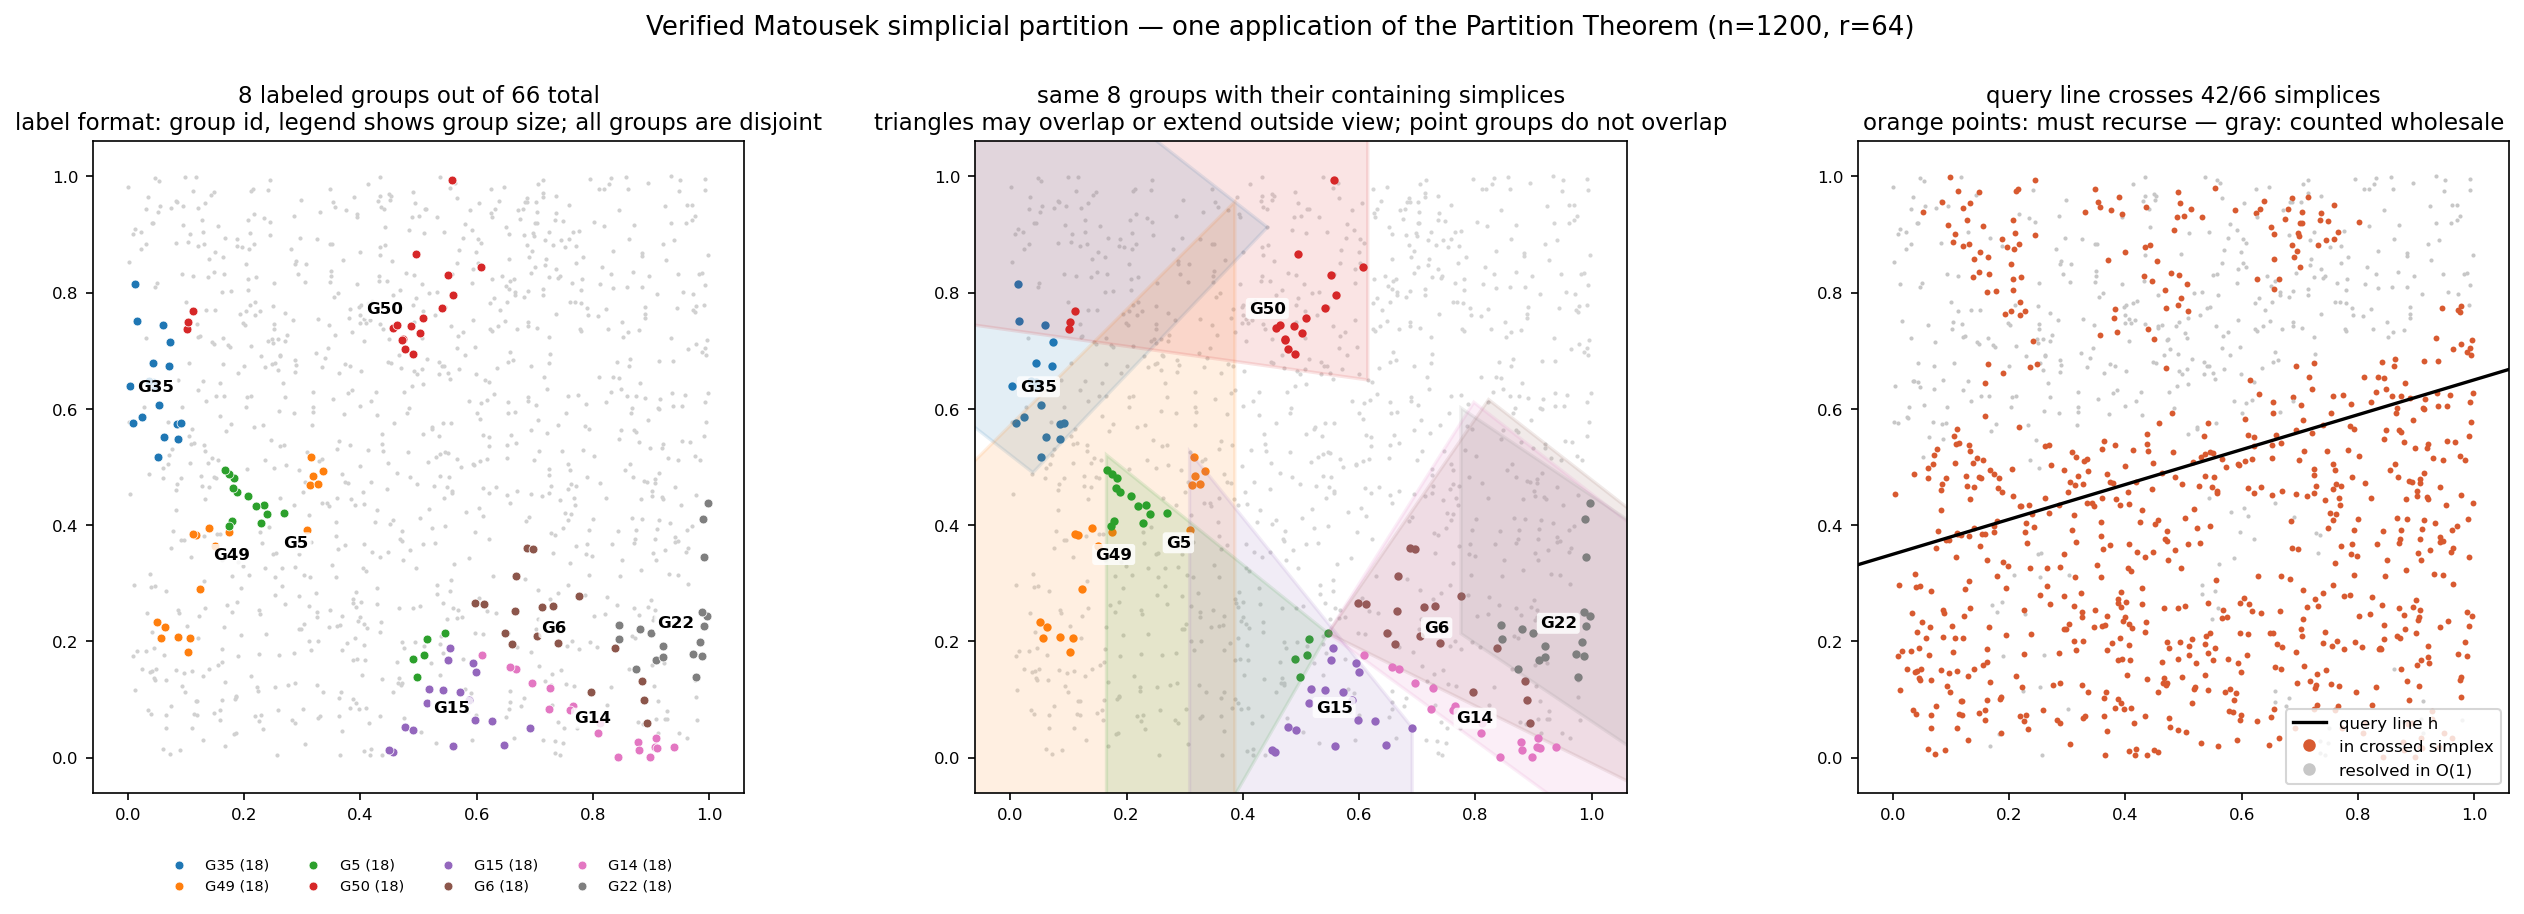
\includegraphics[width=0.8\textwidth]{../assets/partition_tree_example.png}
\caption{One partition step at $n=1200$, $r=64$. Left: representative
  groups. Middle: groups inside their containing simplices. Right:
  groups crossed by one halfplane query versus groups counted
  wholesale.}
\label{fig:partition}
\end{figure}

\begin{figure}[H]
\centering
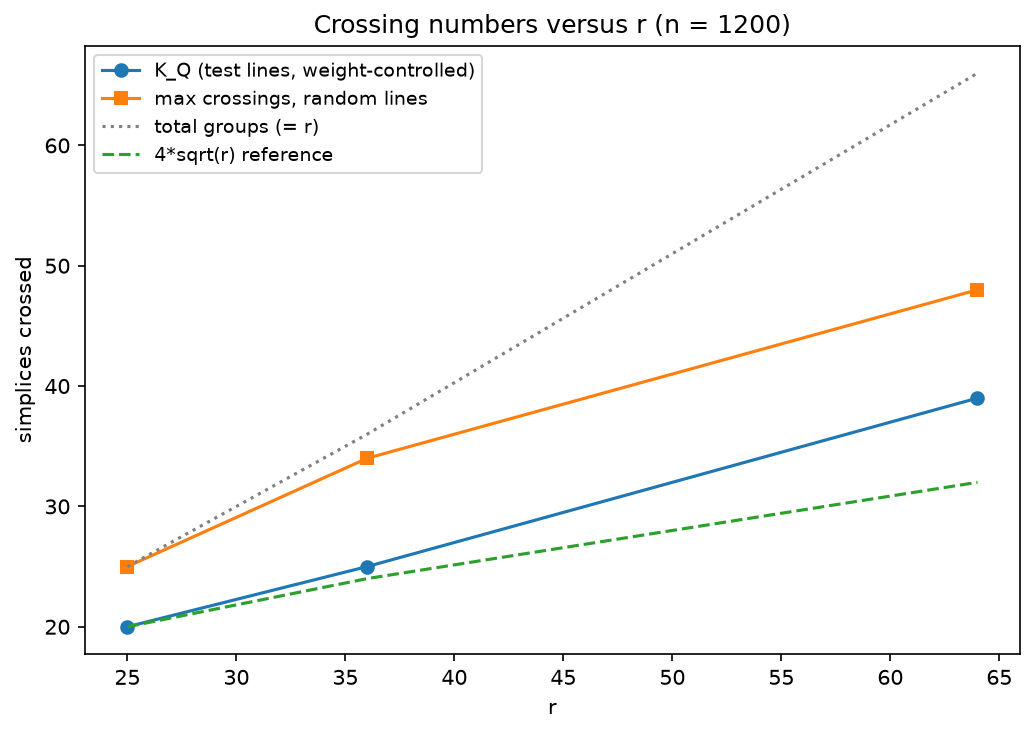
\includegraphics[width=0.62\textwidth]{../assets/crossing_scaling.png}
\caption{Crossing counts as functions of $r$, compared with a
  $4\sqrt r$ reference curve.}
\label{fig:scaling}
\end{figure}

The main observation is simple. The mechanism works: $K_Q$ grows like
$\sqrt r$, with constant about $4$--$5$ in these experiments. But the
transfer bound is still larger than the total group count for all
measured values. With the measured constant, it becomes non-vacuous
only around $r=170$.


\section{Discussion}
\label{sec:discussion}

The experiment shows a theory-practice gap.

The theorem is asymptotically strong. It guarantees that the crossing
number grows like $\sqrt r$, not like $r$. The implementation confirms
that the reweighting mechanism moves in that direction.

The constants are the problem. The measured $K_Q$ is already about
$4\sqrt r$ to $5\sqrt r$. The Test Set Lemma then multiplies this by
3 and adds another $\sqrt r$. For moderate $r$, the resulting bound is
worse than the trivial bound of crossing all groups.

Exact arithmetic also makes the construction slow. At $r=64$, the
construction already takes minutes. The all-lines bound becomes
meaningful only at larger $r$, where this exact implementation is no
longer practical.

This does not contradict the theorem. It explains why practical
spatial indexes often prefer faster structures such as R-trees or
kd-trees, even without the same adversarial guarantee.


\section{Limitations}
\label{sec:limitations}

\begin{itemize}[nosep,leftmargin=*]
  \item The implementation uses a bounding box, not the projective
        plane.
  \item The construction is Las Vegas: bad random choices can fail and
        require retrying.
  \item Very small $r$ values are degenerate for the test-set cutting.
  \item The experiment measures one partition step, not a fully
        recursive range-counting tree.
\end{itemize}

These limitations do not change the main conclusion: the implemented
construction follows the proof mechanism, but the constants are large.


\section{Conclusion}
\label{sec:conclusion}

This report implements the constructive core of Mato\v{u}\v{s}ek's 2D
Partition Theorem and checks the main proof invariants at runtime. The
measured test-set crossing constant is
\[
  K_Q/\sqrt r\approx 4\text{--}5.
\]
The all-lines transfer bound remains vacuous until roughly $r=170$.
So the construction demonstrates the theorem's mechanism clearly, but
also shows why the asymptotic guarantee is hard to turn into a
practical data structure at moderate sizes.

Code, tests, benchmarks, and the longer derivation are available at:
\url{https://github.com/wangyi1010/matousek-partition-tree}.


\begin{thebibliography}{9}

\bibitem{matousek1992}
J.~Mato\v{u}\v{s}ek.
\newblock Efficient partition trees.
\newblock \emph{Discrete \& Computational Geometry}, 8:315--334, 1992.

\bibitem{chazelle1990}
B.~Chazelle and J.~Friedman.
\newblock A deterministic view of random sampling and its use in geometry.
\newblock \emph{Combinatorica}, 10(3):229--249, 1990.

\end{thebibliography}

\end{document}
